% beispiele.tex
In diesem Kapitel werden Beispiele zur Verwendung der R-Paket Funktionen der Faltungskodierung veranschaulicht und erklärt. Kapitel~\ref{kapitel:beispiele_kodierer} führt Variablen ein, die über die weiteren Beispiele hinweg verwendet werden. Die Kapitel~\ref{kapitel:beispiele_kodieren_ohneP} bzw. \ref{kapitel:beispiele_kodieren_mitP} beinhalten die Kodierung und Dekodierung ohne bzw. mit Punktierung. Schließlich werden in Kapitel~\ref{kapitel:beispiele_simulation} Beispiele für die Ausführung von Simulationen vorgestellt. 

\section{Erzeugen von Kodierer und Punktierungsmatrix}
\label{kapitel:beispiele_kodierer}
Vor den Beispielen der Kodierung und Dekodierung werden Hilfsvariablen definiert, die für die folgenden Beispiele verwendet werden. Variablen wie der Faltungskodierer oder die Punktierungsmatrix müssen jedoch nicht unbedingt bei der Kodierung oder Dekodierung mitgegeben werden. Fehlt bei den Parametern der Kodierer wird der Standard-Faltungskodierer aus Beispiel~\ref{bsp:B1} verwendet. Gibt man keine Punktierungsmatrix mit, so wird das Signal auch nicht punktiert. Die meisten weiteren Parameter (Terminierung, Visualisierung etc.) besitzen auch Standardwerte, die verwendet werden, sollten vom Benutzer keine Werte bestimmt werden.
\begin{lstlisting}[caption=Erzeugung von Kodierer und Punktierungsmatrix, label={listing:kodierer_erzeugen}, float=!th]
input <- c(1,0,1,1,0)
 
nasa.encoder <- ConvGenerateEncoder(2, 6, c(171,133))

p.matrix <- ConvGetPunctuationMatrix(c(1,0,1,1,0,1), nasa.encoder)
p.matrix
     [,1] [,2] [,3]
[1,]    1    1    0
[2,]    0    1    1
\end{lstlisting}
Listing~\ref{listing:kodierer_erzeugen} zeigt die Erzeugung der Variablen für die weitern Beispiele. Zunächst wird eine Quellnachricht \texttt{input} erzeugt, gefolgt von der Definition des NASA-Standardkodierers~\cite[S. 90]{morelos2006art}. Zuletzt wird eine Punktierungsmatrix aus dem mitgegebenen Punktierungsvektor und dem verwendeten Kodierer generiert. Der Kodierer ist notwendig, da die Anzahl der Zeilen der Punktierungsmatrix gleich der Anzahl der Kodiererausgänge $N$ ist (siehe Kapitel~\ref{kapitel:grundlagen_punktierung}).

\section{Kodieren und Dekodieren ohne Punktierung}
\label{kapitel:beispiele_kodieren_ohneP}
Im folgenden Beispiel wird eine Nachricht kodiert, verfälscht und sowohl mithilfe der soft decision Dekodierung als auch mithilfe der hard decision Dekodierung dekodiert.
\begin{lstlisting}[caption=Kodierung und Dekodierung ohne Punktierung, label={listing:kodierung_u_dekodierung_ohneP}, float=!tbh]
encoded <- ConvEncode(input, nasa.encoder)
encoded
[1] -1 -1 -1  1  1  1 -1  1  1 -1  1 -1  1  1  1 -1 -1  1 -1 -1  1  1
 
encoded.noisy <- ApplyNoise(encoded, SNR.db = 0.2)
round(encoded.noisy, 2)
[1] -0.83 -0.75 -0.36  1.31  1.05  0.16  0.37 -0.12  1.55 -0.92  3.48 -1.31  0.22  2.49  1.07 -1.19 -1.02  2.00 -1.40 -0.78  1.12  0.50

decoded.soft <- ConvDecodeSoft(encoded.noisy, nasa.encoder)
decoded.soft
$output.soft
[1] -6.67485  6.67485 -6.67485 -6.67485  6.67485

$output.hard
[1] 1 0 1 1 0

decoded.hard <- ConvDecodeHard(encoded.noisy, nasa.encoder)
decoded.hard
[1] 1 0 1 1 0
\end{lstlisting}
Listing~\ref{listing:kodierung_u_dekodierung_ohneP} beinhaltet den Code zur Kodierung und Dekodierung ohne Punktierung. Für die Kodierung der Nachricht wird diese einfach der Kodierungsfunktion \texttt{ConvEncode} zusammen mit dem Kodierer übergeben. Als Resultat erhält man das Kodewort mit den Signalpegeln +1 bzw. -1. Anschließend wird dieses mit der \texttt{ApplyNoise}-Funktion und einem Signal-Rausch-Verhältnis von 0,2dB verrauscht und der \texttt{encoded.noisy} Variable zugewiesen. Die Ausgabe dient dem Vergleich des unverfälschten und des verrauschten Kodeworts. Die Werte werden aus Platzgründen auf zwei Nachkommastellen gerundet. Schließlich erfolgt die soft decision und die hard decision Dekodierung. Der Rückgabewert der soft decision Dekodierung ist eine Liste welche sowohl die Soft-Werte als auch die Hard-Werte beinhaltet. Die hard decision Dekodierung gibt nur einen Vektor mit den \enquote{hart} dekodierten Bits zurück. Das Beispiel zeigt die Fähigkeit der Faltungskodierung, stark verrauschte Signale korrekt dekodieren zu können.

\section{Kodieren und Dekodieren mit Punktierung}
\label{kapitel:beispiele_kodieren_mitP}
Das kodierte Signal kann vor der Übertragung zur Verbesserung der Koderate punktiert werden. Die Punktierung streicht anhand der Punktierungsmatrix Bits aus dem Kodewort, wie in Kapitel~\ref{kapitel:grundlagen_punktierung} beschrieben. Im Folgenden Beispiel wird eine Nachricht kodiert und punktiert bevor sie dekodiert wird.
\begin{lstlisting}[caption=Kodierung und Dekodierung mit Punktierung, label={listing:kodierung_u_dekodierung_mitP}, float=!th]
encoded.punctured <- ConvEncode(input, nasa.encoder, punctuation.matrix = p.matrix)
encoded.punctured
$original
[1] -1 -1 -1  1  1  1 -1  1  1 -1  1 -1  1  1  1 -1 -1  1 -1 -1  1  1

$punctured
[1] -1 -1  1  1 -1  1 -1 -1  1  1 -1  1 -1  1  1

decoded.soft <- ConvDecodeSoft(encoded.punctured$punctured, nasa.encoder, punctuation.matrix = p.matrix)
decoded.soft
$output.soft
[1] -6  5 -5 -5  5

$output.hard
[1] 1 0 1 1 0

decoded.hard <- ConvDecodeHard(encoded.punctured$punctured, nasa.encoder, punctuation.matrix = p.matrix)
decoded.hard
[1] 1 0 1 1 0
\end{lstlisting}
Die Kodierung und Dekodierung mit Punktierung ist in Listing~\ref{listing:kodierung_u_dekodierung_mitP} zu sehen. Die Punktierung erfolgt durch das Mitgeben der Punktierungsmatrix bei der Kodierung. Das Ergebnis der Kodierung ist eine Liste mit dem originalen (nicht punktierten) Signal und dem punktierten Signal. Bei der weiteren Verwendung der Variable ist zu beachten nicht die gesamte Liste zu verwenden sondern das Listenelement des punktierten Kodes. Dies ist beim Aufruf der Dekodierung zu sehen. Die Dekodierung benötigt auch die Punktierungsmatrix für das Auffüllen der punktierten Stellen im Kodewort. Als Ergebnis erhält man wie bei der Dekodierung ohne Punktierung eine Liste der Soft-Werte und Hard-Werte bei der soft decision Dekodierung bzw. einen Vektor der dekodierten Nachricht bei der hard decision Dekodierung.

\section{Simulation}
\label{kapitel:beispiele_simulation}
Die folgenden Kapitel demonstrieren die verschiedenen Möglichkeiten Simulationen durchzuführen. Kapitel~\ref{kapitel:beispiele_simulation_faltungskodierung} beinhaltet ein Beispiel für eine Simulation der Faltungskodierung. Eine Simulation der drei Verfahren der Kanalkodierung des R-Pakets (Blockkodes, Faltungskodes und Turbo-Kodes) wird in Kapitel~\ref{kapitel:beispiele_simulation_kanalkodierung} präsentiert. Kapitel~\ref{kapitel:beispiele_simulation_vergleich} beinhaltet eine Beispielanwendung der Hilfsfunktion zur Darstellung verschiedener Simulationsergebnisse.

\subsection{Faltungskodierung}
\label{kapitel:beispiele_simulation_faltungskodierung}
Das folgende Beispiel zeigt die Ausführung einer Simulation der Faltungskodierung. Die Parameter der Funktion wie der verwendete Kodierer, die Nachrichtenlänge, die zu testenden Signal-Rausch-Verhältnisse, die Anzahl an Wiederholungen je Signal-Rausch-Verhältnis sowie die Punktierungsmatrix können bestimmt werden, sind jedoch auch mit Standardwerten hinterlegt.
\begin{lstlisting}[caption=Simulation der Faltungskodierung, label={listing:ConvSimulation}, float=!th]
> df1 <- ConvSimulation(nasa.encoder, msg.length = 2000, min.db = 0.01, max.db = 0.1, db.interval = 0.01, iterations.per.db = 100)

df1
     db      ber
1  0.01 0.151810
2  0.02 0.140220
3  0.03 0.150020
4  0.04 0.143695
5  0.05 0.142150
6  0.06 0.142900
7  0.07 0.138555
8  0.08 0.137155
9  0.09 0.141615
10 0.10 0.137050
\end{lstlisting}
Listing~\ref{listing:ConvSimulation} zeigt die Simulation mithilfe der \texttt{ConvSimulation}-Funktion. Auf eine Punktierung wird in diesem Beispiel verzichtet. Die Länge der getesteten Nachrichten beträgt 2000. Diese werden bei einem Signal-Rausch-Verhältnis zwischen 0,01dB und 0,1dB verrauscht und im Anschluss dekodiert. Es wird der Mittelwert der Bitfehlerraten über 100 Wiederholungen je Signal-Rausch-Verhältnis gebildet. Der Rückgabewert der Simulation ist ein Dataframe das die Bitfehlerrate (\texttt{ber}) je Signal-Rausch-Verhältnis (\texttt{db}) beinhaltet. Für eine Visualisierung kann der Visualisierungs-Parameter der Funktion gesetzt werden (\texttt{visualize = TRUE}) um einen Simulationsbericht als PDF-Datei generieren zu lassen. Eine weitere Möglichkeit bietet die in Kapitel~\ref{kapitel:beispiele_simulation_vergleich} präsentierte Hilfsfunktion.

\subsection{Kanalkodierung}
\label{kapitel:beispiele_simulation_kanalkodierung}
Für einen Vergleich aller drei Verfahren der Kanalkodierung, die dieses R-Paket umfasst, kann die Funktion \texttt{ChannelcodingSimulation} verwendet werden. Diese Funktion ist eine Wrapper-Funktion, die jede Simulationsfunktion der verschiedenen Kanalkodierungen mit den gleichen Parametern aufruft und die resultierenden Bitfehlerraten in ein Dataframe schreibt und zurückgibt. Das Beispiel in Listing~\ref{listing:ChannelcodingSimulation} führt eine Simulation für eine Nachrichtenlänge von 2000 aus. Die getesteten Signal-Rausch-Verhältnisse liegen zwischen 0,01dB und 0,1dB. Je Signal-Rausch-Verhältnis werden 100 Wiederholungen zur Ermittlung der Bitfehlerrate durchgeführt. Die Dekodierung der Turbo-Kodes erfolgt mit 3 Iterationen. Für eine Visualisierung der Daten kann der Visualisierungs-Parameter der Funktion gesetzt werden (\texttt{visualize = TRUE}) um einen Simulationsbericht als PDF-Datei generieren zu lassen.
\begin{lstlisting}[caption=Kanalkodierungs-Simulation, label={listing:ChannelcodingSimulation}, float=!th]
ChannelcodingSimulation(msg.length = 2000, min.db = 0.01, max.db = 0.1, db.interval = 0.01, iterations.per.db = 100, turbo.decode.iterations = 3)

     db block.ber conv.ber turbo.ber
1  0.01  0.197045 0.088875  0.051680
2  0.02  0.197095 0.088670  0.051570
3  0.03  0.195555 0.090415  0.051935
4  0.04  0.196410 0.089065  0.052815
5  0.05  0.193475 0.089780  0.052700
6  0.06  0.194410 0.090370  0.050620
7  0.07  0.195250 0.089125  0.049625
8  0.08  0.194870 0.086845  0.050740
9  0.09  0.192465 0.089515  0.049495
10 0.10  0.193470 0.084220  0.048935
\end{lstlisting}

\subsection{Vergleich von Simulationen}
\label{kapitel:beispiele_simulation_vergleich}
Das folgende Beispiel zeigt die Ausführung der \texttt{PlotSimulationData}-Funktion. Mithilfe dieser Funktion lassen sich die mit den Simulationsfunktionen erzeugten Dataframes in einem Plot darstellen, was den Vergleich erheblich vereinfacht. In Listing~\ref{listing:PlotSimulationData} wird zunächst ein zweites Dataframe erstellt, welches mit dem in Listing~\ref{listing:ConvSimulation} erstellten Dataframe visualisiert werden soll. Als Vergleich wird ein katastrophaler Faltungskodierer (siehe Kapitel~\ref{kapitel:grundlagen_katastrophale_kodierer}) erzeugt, mit dem die Simulation zur Erzeugung von \texttt{df2} ausgeführt wird. Abbildung~\ref{abb:PlotSimulationData} zeigt den erzeugten Plot.
\begin{lstlisting}[caption=Vergleich mehrerer Simulationsdaten, label={listing:PlotSimulationData}, float=!th]
catastrophic.encoder <- ConvGenerateEncoder(2,2,c(6,5))
df2 <- ConvSimulation(catastrophic.encoder, msg.length = 2000, min.db = 0.01, max.db = 0.1, db.interval = 0.01, iterations.per.db = 100)

df2
     db      ber
1  0.01 0.492040
2  0.02 0.502815
3  0.03 0.490140
4  0.04 0.497805
5  0.05 0.499780
6  0.06 0.489430
7  0.07 0.496505
8  0.08 0.504305
9  0.09 0.493600
10 0.10 0.490645

PlotSimulationData(df1,df2)
\end{lstlisting}
\begin{figure}[!ht]
	\centering
	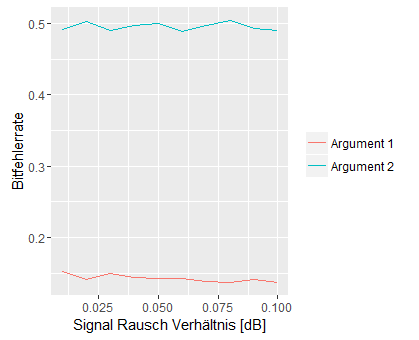
\includegraphics[width=\ScaleIfNeeded]{abbildungen/Rplot_PlotSimulationData}
	\caption{Plot zweier Simulations-Dataframes}
	\label{abb:PlotSimulationData}
\end{figure}